\documentclass[11pt]{article}
\usepackage[a4paper, inner=22.5mm, outer=22.5mm, top=21.21mm, bottom=42.42mm]{geometry}
\usepackage{inputenc}             % to output accented letters and some symbols directly.
\usepackage[english]{babel}       % to set British English.
\usepackage[style=apa]{biblatex}  % APA citation sytle
\usepackage[T1]{fontenc}

% Use "foo" as autoquoting
\usepackage[autostyle]{csquotes}
\MakeOuterQuote{"}

\usepackage{pdfpages} % inlcudepdf
\usepackage{tabularx}
\usepackage{graphicx}
\usepackage{amsmath,amssymb}
\usepackage{lmodern}
\usepackage{hyperref}
\usepackage[title,titletoc]{appendix}


\addbibresource{$bibliography$}

% stolen from pandocs default template. Used for numbered lists
\providecommand{\tightlist}{%
  \setlength{\itemsep}{0pt}\setlength{\parskip}{0pt}}

\begin{document}
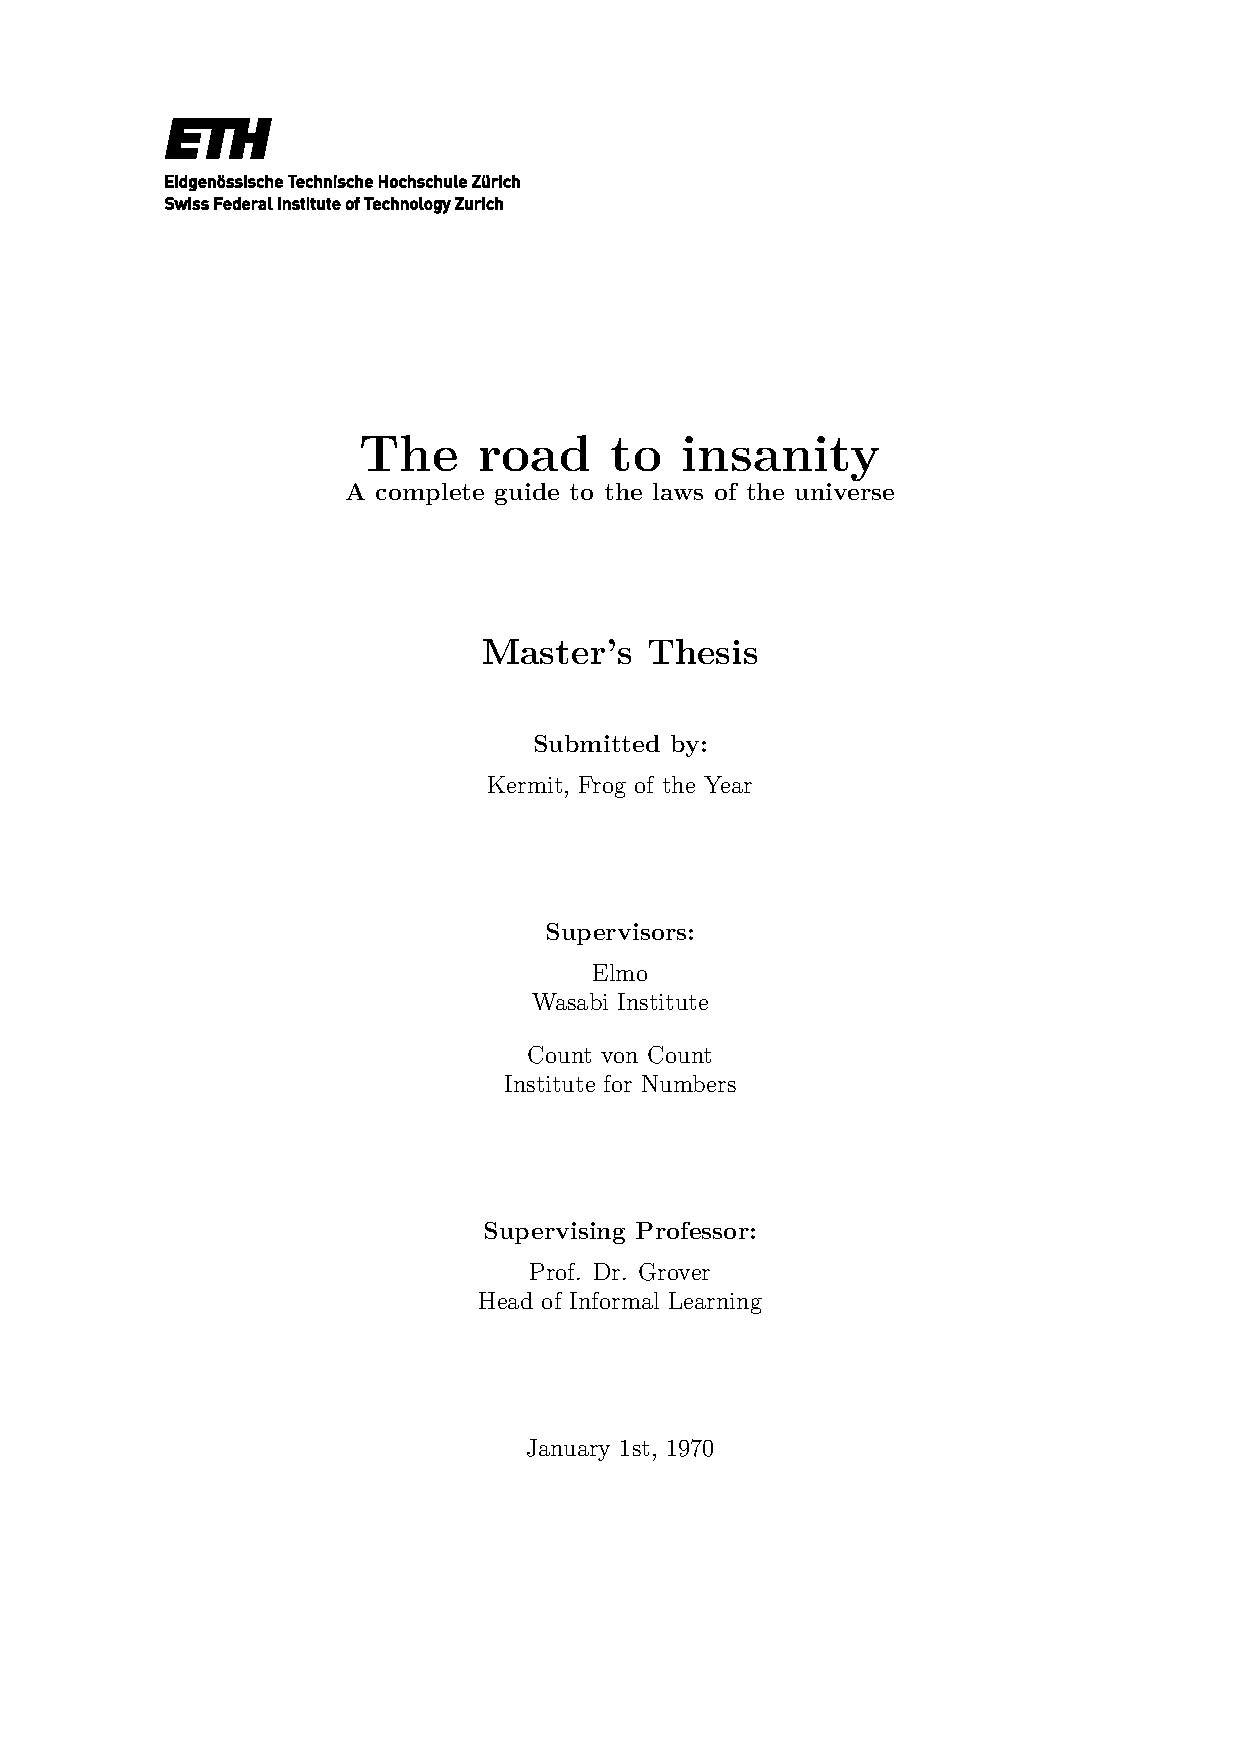
\includepdf{latex/titlepage_eth}
\tableofcontents
$body$ % this will replaced by pandoc
\newpage
\printbibliography[heading=bibintoc,title={References}]
\end{document}

